\chapter{Design} \label{design}

\section{System Overview}
Our wireless stethoscope consists of seven subsystems in order to transfer the auscultation sound signal to a speaker (Fig~\ref{fig:sys_overview}), they are
\begin{itemize}
	\item System power,
	\item Signal sensor,
	\item Signal amplification,
	\item Input circuitry,
	\item Signal processing,
	\item Wireless transmission,
	\item Wired transmission.
\end{itemize}

\begin{figure}[!ht]
	\centering
	
		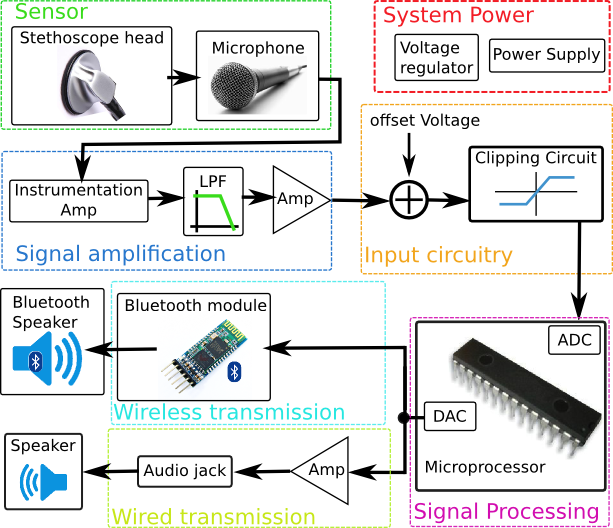
\includegraphics[resolution=120, width=315px, height=315px]{sys_overview2.png}
	
	\caption{System overview}
	\label{fig:sys_overview}
\end{figure}

The sensor consists of a conventional stethoscope head coupled to a microphone, which transforms the sound signal into a voltage signal. This signal is too small to drive any circuitry directly, so it is passed through a signal amplification stage, which results in a bipolar signal. After amplification the signal is passed through input circuitry which introduces a 1.65V offset and limits the voltage to within the maximum tolerable values of the micro-controller in the next stage. This offset is required to transform the signal from bipolar to unipolar, as the micro-controller can not read negative voltages. The micro-controller then performs signal processing in the form of a digital filter, so that it will have the same sound characteristics as a conventional stethoscope. Once processed the signal is transmitted to a Blue-tooth module which transmits the data to a Blue-tooth speaker. In addition an audio jack is available to plug in a speaker directly. All these subsystems are powered by a 9V power source, which can be switched between battery and an AC-DC wall adapter.

\section{System Power} \label{sys_power}
The module is designed to operate in 9V input voltage.  There are two different ways to achieve the required voltage. One option is using a 9V rechargeable battery and the other one is using the 9V DC-wall plug-in adapter.  The two power options provide different benefits when the module is used in different situations. There are some advantages of using a battery. Firstly, using a battery offers true wireless function for users. Secondly, it provides electronic isolation from the main power supply.  In the battery operation, the module is easier to transport and convenient to operate in the outside environment.  A 9V Ni-MH rechargeable battery or any other 9V batteries are suitable for application. A rechargeable battery is ideal because it has less loss when it is not in use. However, the rechargeable batteries could not provide more energy to operate the module for a longer time. From the datasheet of Energizer 9V Rechargeable battery, the battery can operate about 1.2 hours when it discharges at 87.5mA (Fig~.\ref{fig:battery}). The module runs about 80mA.  Thus, the module can last about one hour when a rechargeable battery is used.

\begin{figure}[!tbh]
	\centering
	\fbox{
		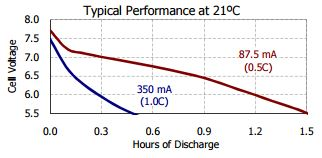
\includegraphics[width=90mm]{battery.jpg}
	}
	\caption{Energizer battery voltage vs. hours of operation\cite{energizer_datasheet}}
	\label{fig:battery}
\end{figure}

Since the energy in a battery is limited, using a wall adapter is ideal when the operating time lasts very long. And it is inconvenient. Wall adapter power supply is the best option when the module needs to be used for a long time indoors.

\section{Voltage Regulation}
In the module, there are two main voltages required (3.3 V and $\pm10$V) .The 3.3V voltage uses to supply the micro-controller and the Blue tooth transmit module while the $\pm10$V voltage used to supply input and output stages’ electronic components.

\subsection{Low Voltage Regulation (3.3V)}
As the input voltage is 9V, buck converter is required to step 9V into 3.3V. LM317L-N 3-Terminal Adjustable Regulator from Texas Instruments provides essential features for the power design (Fig.~\ref{fig:LM317}).  The LM317 can output wide range voltage from 1.2V to 37V and provides large output current up to 100mA. There are another three important functions which are thermal overload protection, current limiting and safe operating area protection. Furthermore, the desired output voltage can be set in a very simple way which requires two external resistors only.  Moreover, LM317 is available in SOIC-8 package and the body size is small enough to satisfy the design requirement. 

\begin{figure}[!tbh]
	\centering
	\fbox{
		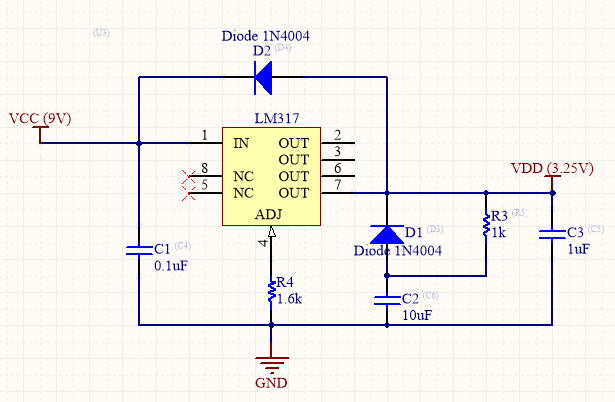
\includegraphics[width=90mm]{LM317.png}
	}
	\caption{LM317 Voltage regulator, schematic taken from datasheet\cite{LM317_datasheet}}
	\label{fig:LM317}
\end{figure}

Circuit with protection diodes is implemented in the module.  According to data sheet, the relationship between output voltage and resistors is showed as follows

\begin{equation}
V_{\textrm{out}} = V_{\textrm{REF}}\left(1+\frac{R4}{R3}\right), \textrm{where } V_\textrm{REF} = 1.25V
\label{eq:LM317}
\end{equation}

Thus, Resistor R3 is chose to 1000 $\Omega$ and Resistor R4 is chose to 1600 $\Omega$ and the output is 3.25 V which is close enough to 3.3V to supply power for micro-controller and Blue tooth module.

In order to preventing the external capacitors from discharging current into the regulator, protection diodes are added to the circuit. The input capacitor C1 and output capacitor C3 are used to reduce the noise in the circuit.  Typical capacitors value can be from 0.1 to 10$\mu$F. 

\subsection{$\pm10$V Regulation}
The module performed well when amplifiers operated in positive and negative 10V when we tested the design. Positive and Negative Voltages are required to generate in the design.

\subsubsection{Choice of Regulator}
The desired voltage ($\pm10$V) can be obtained by a single regulator that can output positive and negative voltage at the same time or two different regulators which generate those voltage separately.  Some inductor-less (Charge Pump) converter can generate positive and negative voltage simultaneously and it only requires capacitors to achieve conversion.  Some switching regulator can generate either positive or negative voltage and it needs to use more components to achieve conversion. One of the inductor-less converters - LT1026 voltage doubler and inverter is considered in the choice (Fig.~). The schematic of LT1026 shows three capacitors could output positive and negative voltage. It operates in a simply way. However, its maximum output current is 15mA. And in our application, it runs about 80mA. After reaching inductor-less converters that we can use, the maximum output current is 100mA. It not very suitable for our application. In contrast, the switching regulator can output very large current which is 200mA or even more. Thus, one boost converter and one voltage inverter are chosen to generate desired voltage. The converters generates large output current and have small output ripple that make the module can operate stably.

\begin{figure}[!tbh]
	\centering
	\fbox{
		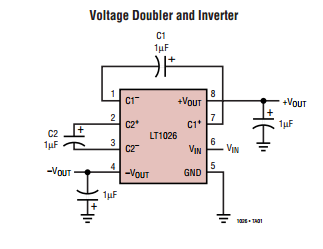
\includegraphics[width=65mm]{lt1026.png}
	}
	\caption{LT1026 Voltage doubler and inverter, schematic taken from data sheet\cite{LT1026_datasheet}}
	\label{fig:LT1026}
\end{figure}

\subsubsection{Positive Voltage Regulation}
Set up DC-DC Converter LT3461 from Linear Technology is used for generate positive 10Voutput voltage.

Then LT3461 setup DC-DC converter is built with an Integrated Schottky and features with small PCB footprint and lower parts cost. The converter operates in fixed frequency -1.3HMz and outputs high voltage up to 36V with wide range input voltage from 2.5V to 16V. Besides, output current is up to 200mA. The predictable output noise due to the constant operating frequency could be easy remove and the switching noise is isolated from input using inductor base topology.

From the typical application circuit (Fig.~\ref{fig:LT3461}) the desired output voltage is set through the feedback pin (Pin 3) with resistors R2 and R3 as follows

\begin{equation}
V_{\textrm{out}} = V_{\textrm{REF}}\left(1+\frac{R2}{R3}\right), \textrm{where } V_\textrm{REF} = 1.255V
\label{eq:LT3461}
\end{equation}

In the application, R2=300k$\Omega$ and R3=43k$\Omega$. Thus, $V_\textrm{out}=1.255\left(1+\frac{300}{43}\right) \approx 10.01V$ and the current goes across R2 and R3 is very small by using larger value R2 and R3. Moreover, 1.5V or higher voltage requires turning on the converter through SHDN Pin (Pin 4). 0.4V or less voltage is used to shut down the converter. RC filter (47k$\Omega$, 47nF) recommended by the data sheet is used and provides soft-start function. Furthermore, output capacitor is charged by inrush current which goes through inductor and Schottky diode. The maximum value of inrush current should be less than 1.5A. The calculation formula is 
\begin{equation}
I_p = \frac{V_i-0.6}{\sqrt{\frac{L}{C}-1}} \exp{ \left( \frac{-\pi}{2\sqrt{\frac{L}{C}-1}} \right)}
\label{eq:inrush_current}
\end{equation}
Where $L$ is the inductance and $C$ is the output capacitance.
In our design, $V_i=9V, L=8.2\mu H, C=6.8\mu F, \textrm{and} I_p=0.5808A$. The peak value of inrush current is in the acceptable range. Besides, the capacitor C3 which is between the output and the feedback pin is phase lead capacitor can decrease the output perturbation and improve transient response. The value is chose to 22pF recommended by the data sheet.

\begin{figure}[!tbh]
	\centering
	\fbox{
		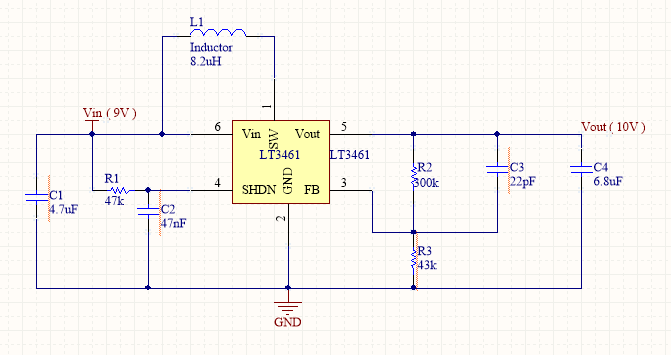
\includegraphics[width=120mm]{lt3461.png}
	}
	\caption{LT3461 typical aplication circuit\cite{LT3461_datasheet}}
	\label{fig:LT3461}
\end{figure}

\subsubsection{Simulation Result}
The operation of converter is simulated by the LTspice (Fig.~\ref{fig:LT3461_ltspice}). Form the simulation, it clearly shows that it takes about 30μs to boost to 10V from 9V input (Fig.~\ref{fig:LT3461_sim}). The output voltage is very flat and stable. It provides stable power supply for amplifiers. 
\begin{figure}[!tbh]
	\centering
	\fbox{
		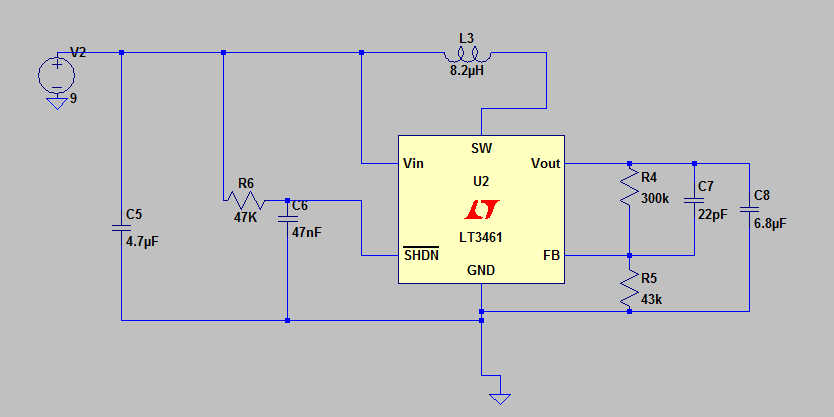
\includegraphics[width=120mm]{lt3461_ltspice.png}
	}
	\caption{LT3461 simulation circuit}
	\label{fig:LT3461_ltspice}
\end{figure}
\begin{figure}[!tbh]
	\centering
	\fbox{
		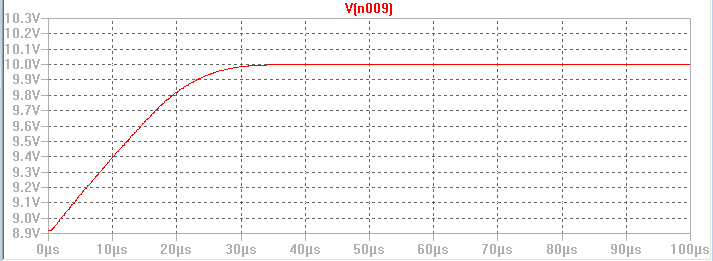
\includegraphics[width=140mm]{lt3461_sim.png}
	}
	\caption{LT3461 simulation results}
	\label{fig:LT3461_sim}
\end{figure}


\subsubsection{Negative Voltage Regulation}
The LT3462, inverting DC-DC Converter, is using the same technology- integrated Schottky Rectifier as the LT3461. The converter operates in 1.2MHz fixed frequency and removes the low frequency noise from the output.  A wide rang input 2.5 V to 16V is suitable for the converter operation and the converter produces high output voltage up to -38V and high output current up to 250mA. Moreover, output voltage can associate with very low output voltage ripple that is approximately 1mV peak to peak. The converter also provides a small footprint and low parts same as The LT3461.
\begin{figure}[!tbh]
	\centering
	\fbox{
		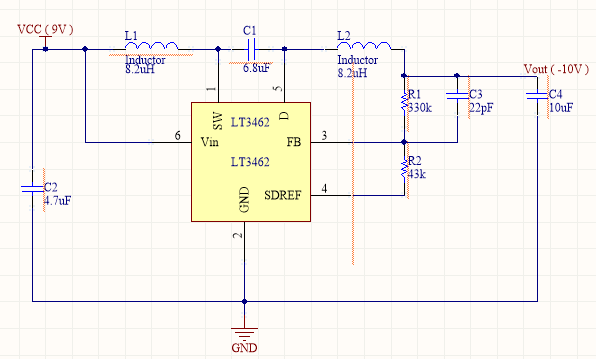
\includegraphics[width=100mm]{lt3462.png}
	}
	\caption{LT3462 typical application circuit taken from datasheet\cite{LT3462_datasheet}}
	\label{fig:LT3462}
\end{figure}
The application circuit of LT3642 showed above is very similar to the typical circuit of LT3641. The required Voltage can be set by Resistors R1 and R2. The relationship is shown as follows
\begin{equation}
R_1 = R_2 \left( \frac{V_{out}}{V_{REF}} \right)
\label{eq:LM3462}
\end{equation}
where $V_\textrm{REF}=1.265V$. In our design, in order minimum the current, large value of resistors are used. R1 is 330k$\Omega$ and R2 is 43k$\Omega$ giving $V_{out} \approx -10V$. The bypass capacitor C2=4.7$\mu$F is used with the input supply pin $V_in$ (PIN6). Furthermore, inrush current which passes through the inductors and the Schottky diode is generated to charge the capacitor to $V_in$ and the peak of inrush current has to be less than 1.5A. The relationship between the peak inrush current, supply voltage, inductors and capacitors is given by the same equation as that for the LT3461 (Eq.~\ref{eq:inrush_current}). Capacitor C1 is known as a ``Flying capacitor'' and requires 1$\mu$F or more. In order to meet those design requirement, the inductors and capacitors are chose to the same as the LT 3461, $L=8.2\mu H, C=6.8\mu F$ And the peak of inrush current is 0.5808A. At last, ceramic type capacitor C4 with value of 10$\mu$F is used to reduce the noise of output voltage.
\subsubsection{Simulation Result}
The converter also can be simulated in LTspice (Fig.~\ref{fig:LT3462_ltspice}). From the simulation, the converter takes about 2ms to reach the desired voltage of -10V (Fig.~\ref{fig:LT3462_sim}). The ripple of the output voltage is very small. It also provide stable system for the amplifiers operation.
\begin{figure}[!tbh]
	\centering
	\fbox{
		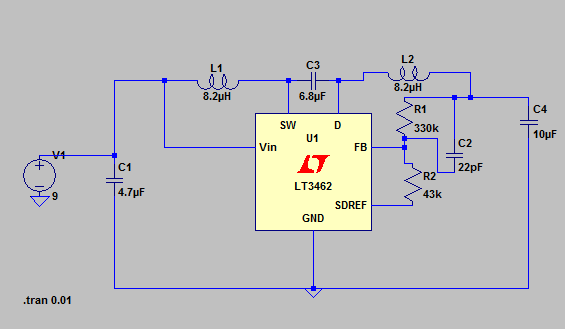
\includegraphics[width=100mm]{lt3462_ltspice.png}
	}
	\caption{LT3462 simulation}
	\label{fig:LT3462_ltspice}
\end{figure}
\begin{figure}[!tbh]
	\centering
	\fbox{
		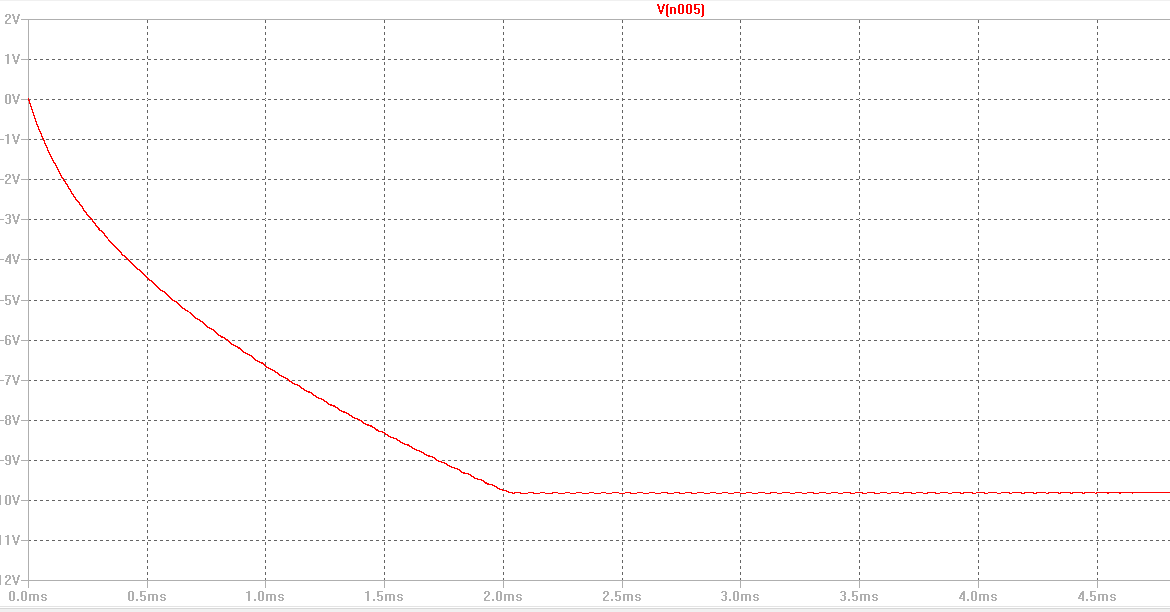
\includegraphics[width=120mm]{lt3462_sim.png}
	}
	\caption{LT3462 simulation results}
	\label{fig:LT3462_sim}
\end{figure}




\section{Signal Sensor}
Our signal sensor consists of a conventional stethoscope head coupled to an electronic sensor. We considered using three different types of electronic sensors to detect the stethoscope sounds, a capacitive, laser and microphone sensor. Capacitive sensors are based on flat-plate capacitors, and can detect a voltage signal between two conducting plates when the distance between them changes\cite[p.104]{Regtien2012} (Fig.~\ref{fig:cap_sensor}). By covering the stethoscope diaphragm in a conductive material it can act as one plate of the capacitive sensor, while a second, smaller plate would have to somehow be mounted inside the stethoscope head. When sound is incident on the diaphragm it causes small vibrations that can then be picked up by the sensor and transmitted as a signal.
\begin{figure}[!tbh]
	\centering
	\fbox{
		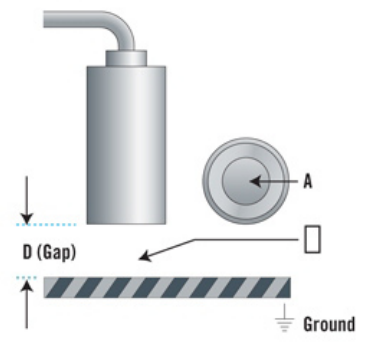
\includegraphics[width=60mm]{cap_sensor.png}
	}
	\caption{Capacitive sensor measuring changes in distance to object, image from MTI instruments\cite{MTI_capsensor}}
	\label{fig:cap_sensor}
\end{figure}
A laser configuration would work by coating the stethoscope diaphragm in a reflective material. When laser light is incident on the material it is reflected to a photo diode within the stethoscope head. This reflected light will be modulated by the small vibrations present on the diaphragm, which contain the sound signal of interest. We can then reconstruct the original sound signal by measuring either the presence, absence or size of the detected beam spot\cite{laserMic} (Fig.~\ref{fig:laser_sensor}).  
\begin{figure}[!tb]
	\centering
	\fbox{
		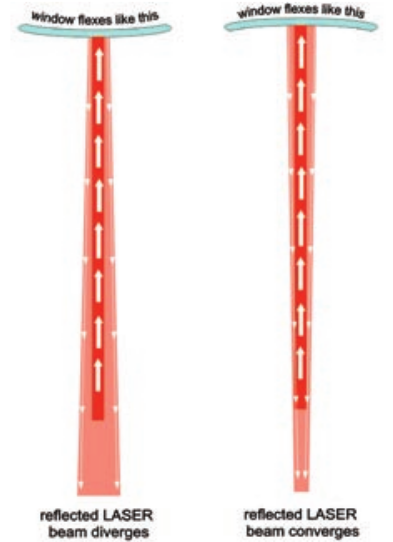
\includegraphics[width=60mm]{laser_sensor.png}
	}
	\caption{Using a laser beam to remotely detect acoustic signals, taken from  Moses \& Trout 2006 \cite{laserMic}}
	\label{fig:laser_sensor}
\end{figure}
The microphone sensor works in a similar manner to the capacitive sensor, however the conducting plates are stored inside a packaged unit (Fig~\ref{fig:mic_condenser}) and it detects sound signals as opposed to the distance to the diaphragm. One of the plates is is made from a very light material and acts as a diaphragm which vibrates when sound waves hit it. As the distance between the capacitor plates changes due to the sound vibrations the capacitance increases (plates closer together) and decreases. This change in capacitance gives rise to a change in voltage and hence an electrical signal. 
\begin{figure}[!tb]
	\centering
	\fbox{
		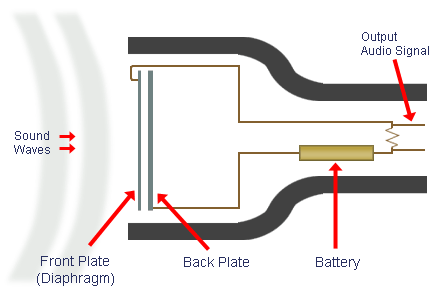
\includegraphics[width=60mm]{mic_condenser.png}
	}
	\caption{Electret microphone}
	\label{fig:mic_condenser}
\end{figure}

We decided to use a microphone sensor because it was the easiest to couple to the stethoscope. All that is required is a small length of the already available stethoscope tubing to attach the microphone to the head. The laser and capacitor sensors however would require either a capacitive plate or photo diode circuit inside the stethoscope head, which has very limited room, making sensor placement a formidable challenge in these cases. We used the POM-5238P-R electret microphone because of its flat response curve for audible frequencies (Fig~\ref{fig:mic_sensitivity}). This means that it wouldn't add any artefacts to the measured sound, such as preferentially transmitting higher frequencies, and so would more closely resemble a traditional stethoscope's sound qualities. In addition it was the most sensitive microphone we could purchase (-38dB) that had a suitable size to couple onto the end of the stethoscope tubing. This high sensitivity would allow us to detect the weak sound signals present within the stethoscope head. The mic signal is obtained by supplying it with a 3.3V source and using a decoupling capacitor to remove the DC component of the device (Fig~\ref{fig:mic_circuit}).
\begin{figure}[!htb]
	\centering
	\fbox{
		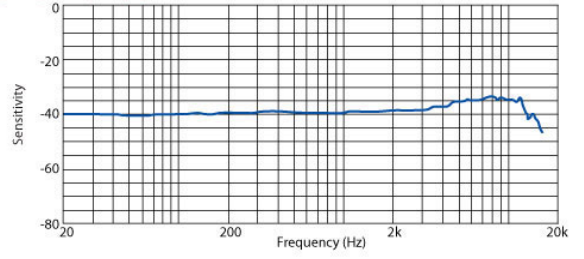
\includegraphics[width=120mm]{mic_sensitivity.png}
	}
	\caption{Plot of POM-5238P-R microphone sensitivity vs. frequency, taken from  data-sheet}
	\label{fig:mic_sensitivity}
\end{figure}
\begin{figure}[!htb]
	\centering
	\fbox{
		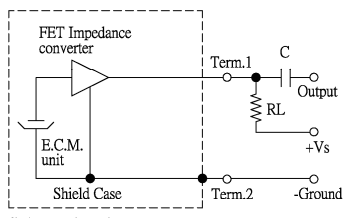
\includegraphics[width=70mm]{mic_circuit.png}
	}
	\caption{Microphone electrical circuit. $V_s=3.3$V from regulator used to power Blue tooth module and microprocessor}
	\label{fig:mic_circuit}
\end{figure}

\section{Signal Amplification}
To amplify the microphone signal we used an instrumentation amplifier, followed by a Low Pass Filter (LPF), and then two non-inverting amplifiers.
The instrumentation amplifier (Fig.~\ref{fig:inamp_circuit}) was used to get an accurate measurement of the microphone signal. It does so because it acts as a difference amplifier with a large Common Mode Rejection Ratio (CMMR), which allows it to significantly reject any noise present on the ground plane\cite[p.~86]{Franco2015}, leaving only the microphone signal. 
\begin{figure}[!htb]
	\centering
	\fbox{
		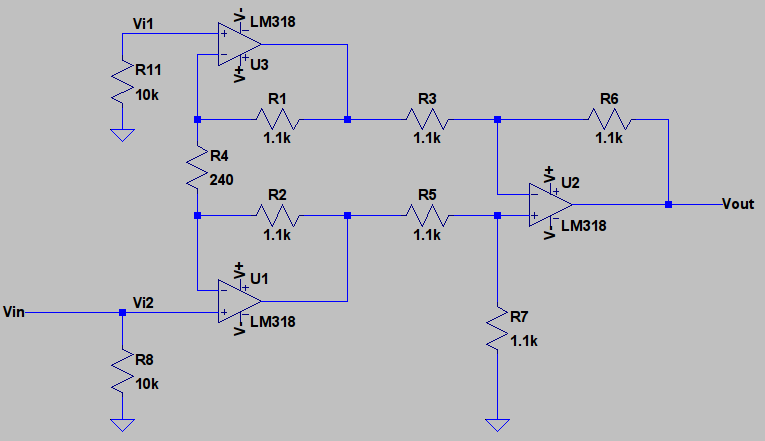
\includegraphics[width=130mm]{instrument_amp_circuit.png}
	}
	\caption{Instrumentation Amplifier circuit used to pick up signal from microphone}
	\label{fig:inamp_circuit}
\end{figure}
This signal is then passed through a LPF to suppress any signal above 20kHz, which is necessary to prevent aliasing in the ADC process of the signal processing stage. The LPF (Fig.~\ref{fig:LPF_circuit}) is implemented by using a second order Sallen-Key configuration\cite[p.~279]{Horowitz1989} and can be designed for different cut-off frequencies through resistor and capacitor values C1, C2, R12, and R13. 
\begin{figure}[!htb]
	\centering
	\fbox{
		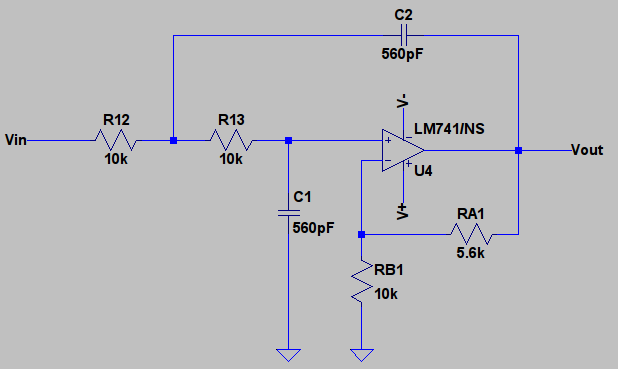
\includegraphics[width=100mm]{LPF_circuit.png}
	}
	\caption{Low Pass Filter (LPF) circuit used to attenuate signals below 20kHz}
	\label{fig:LPF_circuit}
\end{figure}
Finally the two non-inverting amplifiers are used to amplify the signal (Fig.~\ref{fig:amplifier_circuit}). We used two amplifiers in series so that each individual amplifier may have a smaller gain. By having having lower gains the output resistors RA2 and RA3 are smaller, which results in less thermal, or ``Johnson'' noise, and thus a clearer sound signal. We used non-inverting configuration because of its high input impedance. This effectively decouples the design from the preceding LPF stage as it does not load the output, making design of the amplification stage independent from the LPF. 
\begin{figure}[!htb]
	\centering
	\fbox{
		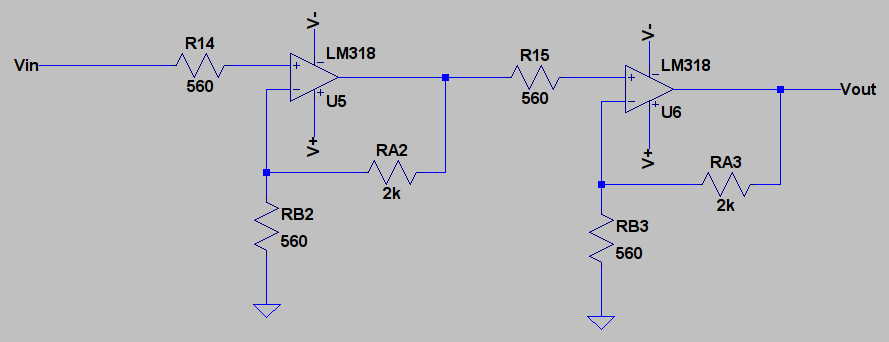
\includegraphics[width=130mm]{amplifier_circuit.png}
	}
	\caption{Amplification circuit used to increase sound signal}
	\label{fig:amplifier_circuit}
\end{figure}
We used LM318 op-amps for the instrumentation and non-inverting amplifiers because of its high gain-bandwidth product (15MHz) and slew rate (50$V/\mu s$), which allows for a larger gain without distorting the signal.

\section{Input Circuitry}
The input circuitry consists of a buffer, summer, and clipping circuit which transform the amplified signal into one that is appropriate for the micro-controller input. The buffer (Fig.~\ref{fig:buffer_circuit}) serves two purposes, firstly it blocks any DC offset introduced from the previous stages, and secondly it decouples these stages from the summing circuit. 
\begin{figure}[!htb]
	\centering
	\fbox{
		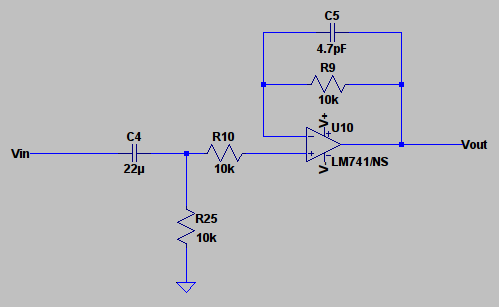
\includegraphics[width=100mm]{buffer_circuit.png}
	}
	\caption{Buffer circuit used to isolate input stage from amplification stage, taken from TI LM318 data-sheet\cite{TILM318}}
	\label{fig:buffer_circuit}
\end{figure}
The summing circuit (Fig.~\ref{fig:summing_circuit}) is used to add 1.65V to the signal. This is necessary because the ADC of the next stage can only accept voltages between 0V to 3.3V, and so can only handle a maximum voltage swing of 1.65V. This summer transforms input signals in the range $\pm1.65$V to the necessary ADC input range and allows for the maximum voltage swing to be measured without clipping, leading to less distortion of the auscultation signal. 
\begin{figure}[!htb]
	\centering
	\fbox{
		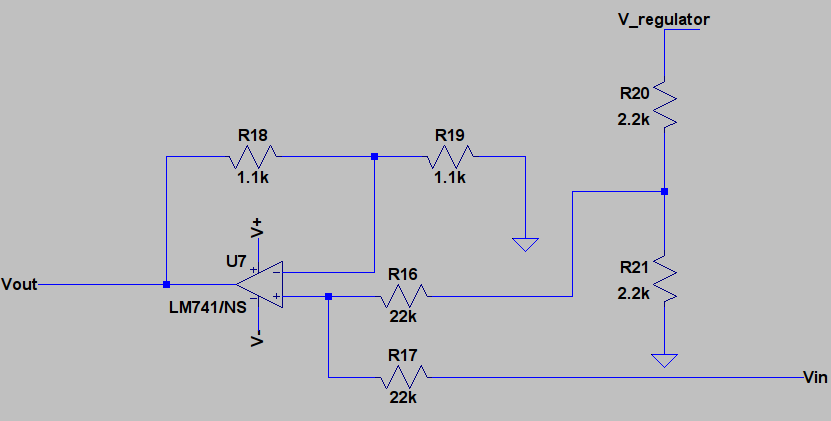
\includegraphics[width=130mm]{summing_circuit.png}
	}
	\caption{Summing circuit used to introduce 1.65V offset of signal coming into the micro-controller}
	\label{fig:summing_circuit}
\end{figure}
Finally the active clipping circuit (Fig.~\ref{fig:clipping_circuit}) is used to protect the micro-controller input. It does so by allowing all signals in the range 0V-3V to pass through, but clips any signal outside this range. This is necessary because it is likely that signals other than auscultation sounds may be amplified, such as the stethoscope diaphragm being knocked as it is placed on the patient. These unwanted signals may cause brief but large signals that could potentially damage the microprocessor input if left unmitigated. Thus the clipping circuit protects the micro-controller input by limiting the voltage passed through.

\begin{figure}[!htb]
	\centering
	\fbox{
		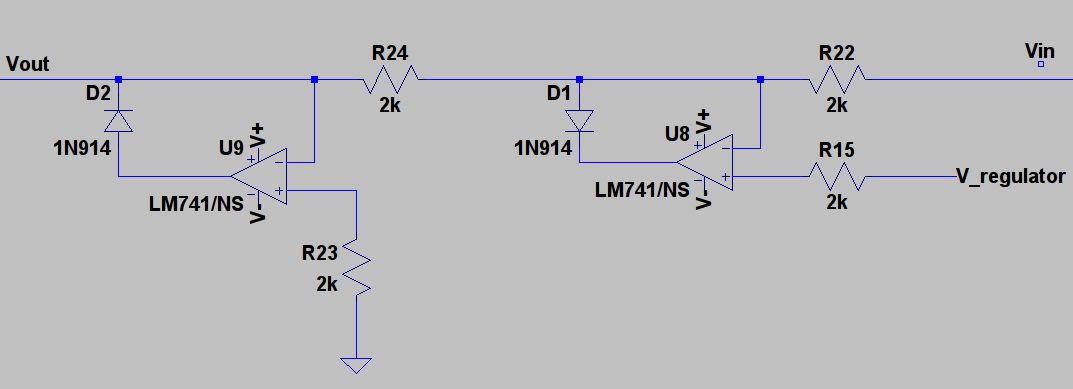
\includegraphics[width=130mm]{clipping_circuit.png}
	}
	\caption{Clipping circuit used to keep input voltage to micro-controller in the range 0-3.3V, taken from \cite[p.~221]{Horowitz1989}}
	\label{fig:clipping_circuit}
\end{figure}

We used an LM741 op-amp for all the circuits in the input-stage because it is the cheapest op-amp we know of. Its unity gain bandwidth of 1MHz is sufficient because these circuits don't amplify the signal, they only pass it through. By using these cheaper, ubiquitous op-amps we lower the cost of the overall system. 

Note that both the summing and clipping circuit also require the regulated 3.3V ($V_\text{regulated}$) to function, which is taken from the LM317 voltage regulator that is also used to power the microphone, Blue-tooth module, and micro-controller (Section~\ref{sys_power}).


\section{Signal Processing}
A micro-controller processes the sound signal using Infinite Impulse Response (IIR) and Finite Impulse Response (FIR) digital filters. This signal processing is used to filter out unstable feedback frequencies and to reproduce the sound characteristics of a conventional stethoscope. Unstable feedback occurs when the microphone sensor picks up the sound played through the speaker. It happens at specific resonant frequencies which depend on the length of the coupling tube, stethoscope diaphragm, and microphone (section \ref{feedback-freq}). If left untreated these unstable frequencies can grow in amplitude until the user can only hear a large squealing sound from the device, making auscultation impossible. The micro-controller further processes the signal in order to negate the effect that having a smaller coupling tube has on the transmitted sound. The tube length of the original stethoscope is approximately 50cm, while our design has a coupling tube of only 3cm. This difference in length changes the sound transmission properties of the tube, dampening sound frequencies by a different amounts. Negating this ``colouration'' effect helps reproduce the type of sounds doctors currently listen for with a conventional stethoscope.

\subsection{Microprocessor Requirements} \label{mcu-requirements}
In order to decide which microprocessor to use we need to first establish the minimum requirements. We consider the bus size, speed, and the amount of working memory needed to implement the digital filters.

Bus sizes for microprocessors generally come in 8, 16, and 32-bit. This bus size determines the bit-depth, which is number of bits stored per sample. A larger bit-depth will require more memory to store samples, however it will suffer less quantization noise, which is the result of truncation error inherent in ADC. For our system we used 16 bit bit-depth because that's the same used in CDs~\cite[p.~27]{Schroder2011}, and we assumed CD audio quality would be sufficient.

To determine how fast the processor needs to be we estimate how many Million Instructions Per Second (MIPS) that it has to execute. To perform this calculation we need the sampling frequency ($F_s$) and the order of the digital filter we wish to implement ($N$). We take $F_s$ to be 40kHz, the Nyquist frequency associated with 20kHz sounds. Although we require to capture sounds only up to 4kHz (Section~\ref{max-sound-freq}) we use the more conservative figure for flexibility to change the design in the future. The order of the filter $N$ was unknown at the time of purchasing the micro-controller, hence an estimate of $N=100$ is used, as our past experience with designing low pass digital filters found this to be a conservative estimate. $N^{th}$ order digital filters are typically calculated as~\cite[p.~164]{Mitra2011}
\begin{equation}
y[n] = p_0 x[n] + p_1 x[n-1] + \cdots + p_N x[n-N] - d_1 y[n-1] - \cdots - d_n y[n-N]
\label{eq:filter}
\end{equation}
where $y$ is the sampled output signal, $x$ is the sampled input signal, and $d_i, p_i$ are constant filter coefficients. This requires $2N$ additions and $2N$ multiplications, for a total of $4N$ instructions per output sample $y[n]$. In addition to the digital filter the controller must also transmit 16 bits of data per sample to the Blue-tooth module, giving a required speed of $(16+4N)F_s=(16+400)40\cdot10^3=16.64$ MIPS. Thus if we round up for safety then we require a processor capable of at least 17 MIPS.

The amount of working memory required is calculated by noting that the filter in Eq.~\ref{eq:filter} needs to store $2(N+1)$ coefficients $(p_i, d_i)$, $N+1$ input signal samples $(x)$ and $N+1$ output signal samples $(y)$, for a total of $4(N+1)=404$ 16 bit values, or 808 Bytes of RAM. We round this value up to the nearest KByte and double it as a safety margin to get a minimum requirement of 2KBytes of RAM.

In summary our micro-controller needs to be at least 16-bit, capable of 17 MIPS with at least 2KBytes of working memory.

\subsection{Microprocessors Considered}
We considered five microprocessors for the system, the Arduino nano, Raspberry Pi, ADSP-BF504 Blackfin processor from Analog Devices, and the dsPIC33-FJ64GP802 from Microchip. Each processor was scored in terms of its coding, interface, size, speed, and cost, and a weighted total score determined which processor to use. 

Coding relates to what programming language the processor can be coded in. Languages such as C and Python are considered higher level than Assembly for example, and are more desirable to code in because it is quicker to develop in these languages, which will help us meet the time constraints of the project. 

Interface describes how easy it is to upload a program to the device. We wish to have the unit programmable while in a circuit in order to minimise the time it takes to debug the hardware and software. If it has to be disconnect or unplugged from our circuit for each upload iteration this could be prohibitively time consuming. 

The size of the processor will affect the size of our stethoscope. If it is too large to be comfortably held in the hand then it will not have met its specifications, thus we require a processor that won't greatly increase the size of our final design.

Speed is constrained to be at least 17 MIPS (Section~\ref{mcu-requirements}), anything above this is considered a bonus as it allows for further flexibility in filter design. 

Finally we considered cost, by minimising the processor cost we minimise the cost of our final device and thus the likelihood of it being used or purchased.

From our weighted total scores we decided to use the dsPIC33-FJ64GP802 microprocessor (Table~\ref{mcu-decision-matrix}). In our scoring analysis we estimated the speed to be the clock frequency of the device, which meant the Adruino was not fast enough to perform the required filtering computation. The Raspberry pi provided the greatest speed however it was both the largest and most expensive option, which made it less feasible. The Blackfin BF504 also provided considerable speed however it was only sold in surface mount packages or as part of a development board, making it difficult to prototype onto a bread board. Thus because of its low cost, small form factor, and ability to handle the required computation we decided to use the dsPIC.
\begin{table}[htbp]
\caption{Microcontroller decision matrix}
\begin{center}
\begin{tabular}{rccccc}

\hline
\multirow{2}{*}{\textbf{}} & 
\multirow{2}{*}{\textbf{weight}} & 
\textbf{\small{Arduino}} & 
\textbf{\small{Raspberry}} & 
\textbf{\small{AD}} & 
\multirow{2}{*}{\textbf{\small{dsPIC}}} \\ 


 & & \textbf{\small{(nano)}} & \textbf{\small{pi}} & \textbf{\small{Blackfin}} & \\

\hline

\textbf{Coding} & 7 & 10 & 10 & 10 & 10 \\ \hline

\textbf{Interface} & 10 & 10 & 10 & 1  & 10 \\
& & \multicolumn{2}{c}{\small{(USB cable)}} & \small{(dev board / SMD)} & \small{(programmer)} \\
\hline

\textbf{Size} & 9 & 7 & 5 & 10 & 10 \\
& & \small{(3cm$\times$5cm)} & \small{(10cm$\times$15cm)} & \small{(1.2cm$\times$1.2cm)} & \small{(0.7cm$\times$3.6cm)} \\
\hline
 
\textbf{Speed} & 6 & 0 & 10 & 9 & 7 \\
& & \small{(16MIPS)} & \small{(700MIPS)} & \small{(400MIPS)} & \small{(40MIPS)} \\
\hline

\textbf{Cost} & 8 & 6 & 4 & 5 & 10 \\ 
& & \small{(\$20)} & \small{(\$30)} & \small{(\$25)} & \small{(\$5)}\\
\hline

\multicolumn{2}{r}{\textbf{\footnotesize{Total weighted score}}} & \textbf{281} & \textbf{307} & \textbf{264} & \textbf{382} \\ \hline
\end{tabular}
\end{center}
\label{mcu-decision-matrix}
\end{table}


\subsection{dsPIC33 micro-controller}
\subsubsection{Features}
We used a dsPIC33-FJ64GP802 microprocessor to process the sound signal. The chip contains an ADC, audio DAC and dedicated Digital Signal Processing (DSP) engine, which make it well suited to filter our signal. The DSP engine (Fig.~\ref{fig:dsp_block}) is capable of retrieving two words of data from memory, multiplying them and summing them to a running total in a single instruction cycle. This operation of Multiplying and ACcumulating (MAC) is frequently used in digital filters, and so being able to perform a MAC in a single cycle makes the chip efficient for our purposes. The ADC is capable of converting 500k 12-bit samples per second through successive approximation conversion, so it is fast enough to handle our maximum requirement of 40k samples per second. ADC conversions are also written directly to memory, without any CPU intervention, through the chip's Direct Memory Access (DMA) feature, resulting in less overhead and allowing the chip to execute more instructions per sample. Finally the DAC is designed specifically for audio applications, and is capable of producing up to 40kHz signals, making it suitable for our application as we wish to output a filtered sound signal. 

\begin{figure}[!ht]
	\centering
	\fbox{
		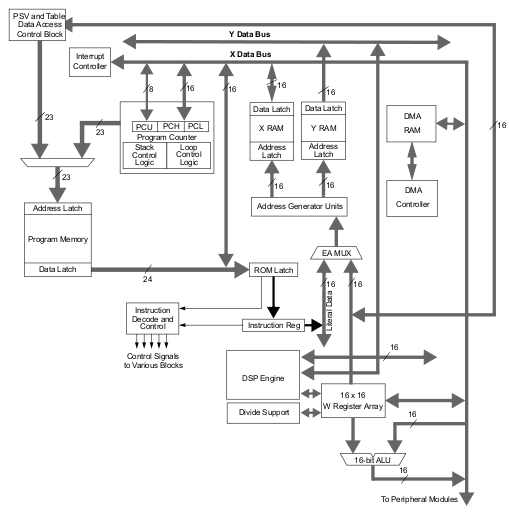
\includegraphics[width=150mm]{dsp_engine2.png}
	}
	\caption{Micro-controller with DSP-engine and two address generator units to pre-fetch data for Multiply and Accumulate instruction (MAC). Taken from dsPIC33F data-sheet \cite[p.~14]{dspic_datasheet}}
	\label{fig:dsp_block}
\end{figure}

\subsubsection{Operation}
The dsPIC utilises two memory locations, buffers A and B, to apply the digital filter. In one cycle the ADC writes to buffer A, while the filter function operates on data in buffer B and outputs the result to the DAC (Fig.~\ref{fig:mcu_operation}). In the next cycle the ADC writes to buffer B while the filter is applied to buffer A samples. This ``ping-pong'' switching between the two buffers allows the ADC to sample data while the dsPIC simultaneously applies a digital filter to previous data samples, which results in a continuously filtered output signal. The filter is executed using the IIR and FIR functions of the DSP library that is included with Microchip's dsPIC Integrated Development Environment ``MPLABX''.

It is important to assure that the rate at which buffer's A and B are written to by the ADC and read from by the DAC are synchronized, otherwise the output signal will be distorted. If the ADC writes data at a different rate than the DAC reads it then the output signal will be shifted in frequency compared to the input signal. It is also possible for newer input samples to overwrite previous ones before they've been processed, corrupting that block of data. The time at which the ADC samples is controlled by an internal counter. The counter raises an interrupt after a programmed number of system clock cycles, which gives us great flexibility in setting the ADC sampling frequency. The DAC clock however is constrained to run off an auxiliary clock, scaled down by a selectable factor from between 1 to 128, which restricts what sampling frequencies we can use the most. Hence our sampling frequency for the system was set to 48kHz in order to satisfy the ADC/DAC synchronization condition.

\begin{figure}[!htb]
	\centering
	\fbox{
		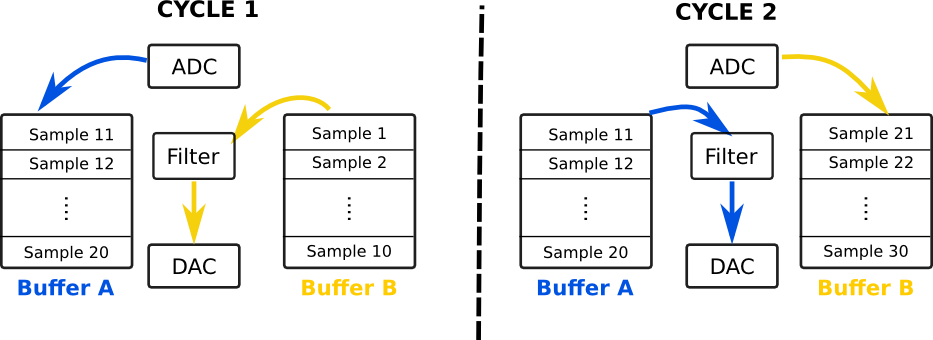
\includegraphics[width=130mm]{mcu_operation2.png}
	}
	\caption{Micro-controller uses two memory buffers to simultaneously sample and filter sound data}
	\label{fig:mcu_operation}
\end{figure}



\subsection{Micro-controller Audio output}
The microchip provides a 16-bit Delta-Sigma signal Digital-to-Analog converter for audio application.  The Left and Right channels are used in the audio operation. In our application, only one channel is used. The DAC output has two analog voltages, a Positive DAC output and a Negative DAC output, for each output channel.  An external circuit is required to provide a single end output.  A simple op amp differential amplifier circuit is designed to achieve the purpose. 

\begin{figure}[!htb]
	\centering
	\fbox{
		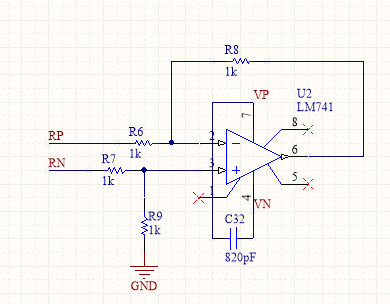
\includegraphics[width=90mm]{DAC_OUT.png}
	}
	\caption{Operational amplifier used for micro-controller single ended output, circuit taken from DAC data sheet\cite{DAC_datasheet}}
	\label{fig:dac_output}
\end{figure}

An op amp differential amplifier built with negative feedback provides predictable and stable gain for output (Fig.~\ref{fig:dac_output}). RP is Positive DAC output and RN is Negative DAC output.  All the resistors are the same and the gain is 1 for the output.  The general purpose operational amplifier LM741 from TEXAS INSTRUMENT is used in the application. A decoupling capacitor C32 820pF is used to bypass the power supply to reduce the noise caused by the other circuit elements. 


\section{Wired Transmission}
The output voltage from microcontroller is maximum 1V peak to peak with 1.5V DC offset. The signal is too weak and hard to be listened through the speaker. Another amplification stage is required to amplifier audio signal.
The low voltage audio power amplifier LM386 is adopted in this amplification stage. The LM386 is ideal for battery operation with wide voltage range from 4V to 12V. It is easy to operate. Low distortion is approximately 0.2\% and the quiescent current drain is roughly 4mA. Application circuit minimums external parts to adjust the gain from 20 to 200.  It is available in 8 pin MSOP package. Its size is small enough to suit PCB board. And it is ideal for low voltage sound system application.
\begin{figure}[!htb]
	\centering
	\fbox{
		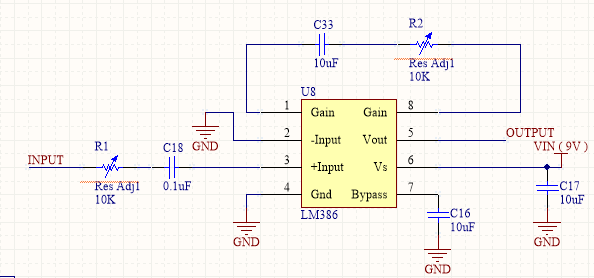
\includegraphics[width=110mm]{LM386.png}
	}
	\caption{LM386 typical application circuit taken from data sheet\cite{LM386_datasheet}}
	\label{fig:LM386}
\end{figure}
The power supply pin (Pin 6) of LM386 directly connects to the power supply (9V) bypass decoupling capacitor to operate. The audio signal goes into the input pin (Pin 3) through a variable resistor which is up to 10k$\Omega$ and a capacitor. The volume of output signal can be change by changing the value of the variable resistor.  Besides, the LM386 provides flexible gain control functions using two simple pins Pin 1 and Pin 8. Leaving pin1 and pin 8 open, the gain at 20 is provided. When a capacitor is placed between those two pins, the gain goes to 200.  Moreover, in the application, a variable resistor and a capacitor are placed in series and the gain can be varied from 20 to 200. 

\section{Wireless Transmission}
Wireless transmission is implemented using Blue tooth technology. The Blue tooth Module we used is an integrated circuit based on the CSR8605 chip. CSR8605 is baseband IC for Blue tooth.  It features with 2.4 GHz systems and Blue tooth low energy. It also supports Blue tooth v4.0 specification, AVRCP v1.0 and A2DP v1.2 Blue tooth profiles. Wide range physical interfaces are provided.  Those are UART interface for debug, USB 2.0 interface, SPI interface, PCM and I$^2$C interface (Fig.~). The integrated audio codec is included in the chip to meet a variety of audio standard. The Kalimab DSP coprocessor supports most of the audio and DSP application. 

\begin{figure}[!htb]
	\centering
	\fbox{
		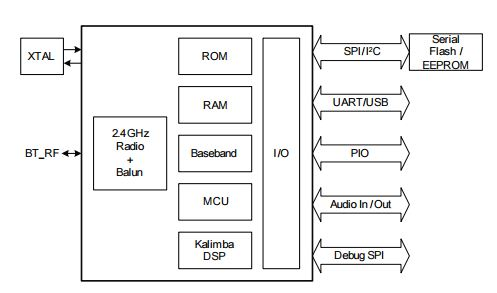
\includegraphics[width=100mm]{bluetooth_block.jpg}
	}
	\caption{Blue tooth module interfaces taken from data sheet\cite{Bluetooth_datasheet}}
	\label{fig:bluetooth_block}
\end{figure}

\subsection{Integrated Blue tooth Module}

\begin{figure}[!htb]
	\centering
	\fbox{
		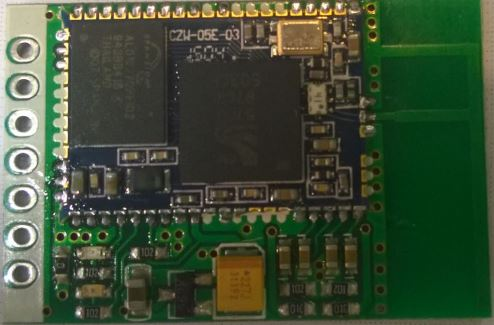
\includegraphics[width=80mm]{bluetooth_module_photo.jpg}
	}
	\caption{Photograph of Blue tooth module}
	\label{fig:bluetooth_photo}
\end{figure}

The Integrated Blue tooth Module operates by DC supply voltage from 3 to 4.2 V and output current is approximately 13mA Max.  The transmission distance is up to 10 meters. Two analogy inputs, Left and Right Channels, are provided. The Blue tooth Module will pair with Blue devices which have default paired pin words such as “000”,”1234”,”1111” and “8888”. Besides, it will send request to pair the most recent paired blue device once it turns on.  During the paring model, the red and blue LED will flash quickly. And only the blue LED will flash slowly after paring model. The Blue tooth Module will automatically turn off if it does not pair any blue devices in 10 minutes. The Blue tooth Module is easier to implement, with seven headersare provided (Fig.~\ref{fig:bluetooth_photo}). The module is simply operated by connecting the corresponding pins (Fig.~\ref{fig:bluetooth_connection}). Analog inputs connect directly into Left and Right channel pin since only one channel is used in our application. Two resistors are connected to LED pins and it reduces the current in the module. And the supply voltage is from the 3.3V regulator.

\begin{figure}[!htb]
	\centering
	\fbox{
		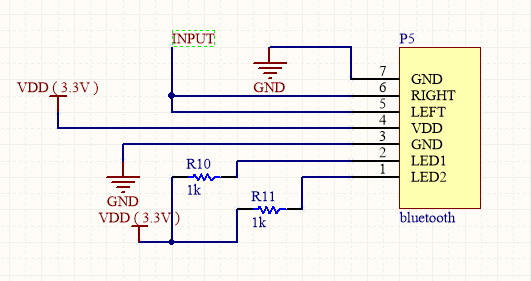
\includegraphics[width=80mm]{bluetooth_schematic.png}
	}
	\caption{Schematic for interfacing with Blue tooth module}
	\label{fig:bluetooth_connection}
\end{figure}


\section{PCB Management}
All the electronic elements are soldered onto a Printed Circuit Board (PCB). The size of the application PCB is about 15 cm length and 5 cm wide (Fig.~\ref), and can be covered by a plastic cylinder that it is easier for users to hold it in their hands. There are four holds on the each corners that use to make the PCB stable when it is covered by a plastic cylinder.

The microphone is located on the left centre of the PCB. This makes it easier to attach stethoscope diagram with the microphone. Each input stage is then placed from left to right. The DSP controller is vertically placed in the middle of the PCB and the output stages locate on the right side of the controller. Each stage is connected through two pin headers, which are all placed horizontally bottom of PCB. This way we can disconnect any stages if it fails or add other stages in the future.

On right side of the controller, there are three LEDs – RED, GREEN, BLUE which indicate the power, DSP working and the Blue tooth Module operation. Two switches are placed next to the LED on the right corner. One is power switch and another is Blue tooth switch. Then the Blue tooth module is placed blew the switches and in the middle of the PCB while the audio jack is placed under the Blue tooth module. Finally the power plug is located on the right end of the PCB and the battery holder on the under side of PCB behind the Blue tooth module.
\begin{figure}[!htb]
	\centering
	\fbox{
		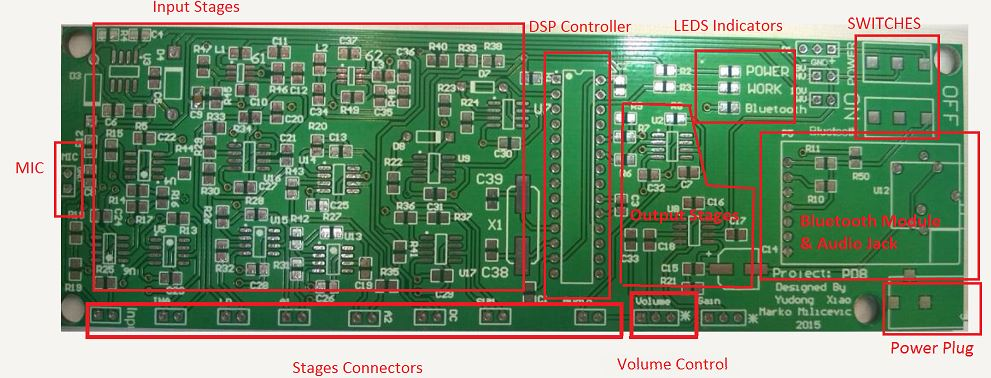
\includegraphics[width=145mm]{pcb_top.jpg}
	}
	\caption{PCB used to hold electronic components}
	\label{fig:pcb}
\end{figure}